% !TEX root = ../main.tex

\chapter{绪论}
\label{chap:intro}

\section{课题研究背景及意义}
\label{intro:sec:bg}

空战往往在现代战争中扮演着决定性的作用,在近年几次世界局部冲突中充分体现出制空权的重要性,而随着各国军事技术的发展,空战的无人化、集群化、智能化是一个必然的趋势,如在今年的亚美尼亚与阿塞拜疆的纳卡地区冲突中,阿塞拜疆的无人机作战对亚美尼亚造成了巨大杀伤。除了无人机以外,空空导弹作为空战中的一种高威胁高杀伤力武器,如果能将其实现集群化智能化攻击,则会大大增加空战取胜的概率,向军事现代化、智能化迈出重要一步。

空空导弹实现集群智能作战的关键技术包括协同探测技术、协同决策技术、协同制导技术等,贯穿了导弹从发现到打击目标的全流程。其中,空空导弹的协同决策系统是重中之重,其主要功能时负责导弹集群的任务分配,这里的任务可以包括目标的分配,可以是侦查、打击、评估等多任务分配,或者是子集群的划分。任务分配的目标可以概括为:在当前态势环境下对我方资源进行调配以实现我方效益的最大化。随着军事技术的发展,尤其是集群化作战规模逐渐增大的发展趋势,协同决策系统中的任务分配技术的重要性越来越突出,一方面拥有自主决策系统的导弹可以共享态势信息,从而更好地应对快速变化的空战态势,及时根据态势信息选择最优策略,最大化攻击效益。另一方面,虽然空空导弹经历了几代发展,已经具备了全向攻击的能力,但在实战中导弹的命中率仍然受发射条件和目标特性影响较大,尤其是最新一代战机在机动能力、隐身能力和干扰能力方面不断取得进步,为空空导弹的攻击带来了一定的难度。此时协同决策系统可提前布局,为导弹预先选好最优目标,尽量让所有导弹向着有利于命中目标的方向靠拢,从而提高导弹的整体打击效果。

针对任务分配问题,大量研究成果针对不同场景提出了各式各样的任务分配模型和算法,这些方法按照架构主要分为集中式和分布式。典型的集中式任务分配模型是混合整数规划模型(Mixed Integer Linear Programming, MILP),将任务分配问题视为一种组合优化问题。MILP模型下常用的集中式算法包括匈牙利算法、分支定界法,以及各种启发式优化算法及其改进版本。这些算法下智能体大多没有自主性,只是服从决策中心作出的最优决策,因此本质上说没有体现协同的作用,且集中式算法在大规模集群中的性能也有明显的下降。

相对于集中式算法,分布式算法赋予了各智能体一定的自主性和决策能力,因此具有如下优势:(1)使得集群计算负载能够相对均衡地分配到各个节点上;(2)对于部分连通或时变网路具有更好的鲁棒性;(3)不需要一个集中的数据收集处理中心,更适用于大规模集群;(4)响应迅速,面对态势变化,分布式架构下各导弹可以立即自行调整策略,及时响应。

但在实际空战场景中,由于受到空空导弹自身、任务目标需求及空战环境等因素的制约,空空导弹的分布式任务分配算法仍然是一个非常复杂的问题,其复杂性主要体现在以下几个方面:

(1)空战环境的复杂性。随着科技的发展,世界先进的导弹和战机都具备了高速高机动能力,且即使在恶劣天气下,也可全天时、全天候作战,这使得空空导弹作战的环境日趋复杂化,使得导弹难以对变化的态势及时作出响应;

(2)目标的异构性。集群作战,如战机集群,往往是由不同种类、不同分工的飞机组成,如一架预警机与多架战斗机组成的侦查护卫编队。因此在任务分配中需要考虑不同类型目标的差异,指派合适的导弹进行攻击;

(3)分布式架构的局限性。分布式架构下,一方面导弹间通信链路往往也是分布式的,受通信带宽和通信频率的限制,导弹获得信息可能是非同步、非一致的,这对任务分配问题带来了很大的困难;另一方面,以目标分配为例的任务分配问题本质上是一个组合优化问题,这是一个典型的NP-hard问题,在求解该类问题时,分布式优化算法相比于集中式算法仍存在着优化效果不好的缺点,尤其是在导弹仅能获得局部信息的前提下,如何获得全局最优仍是一个开放的问题。

目前分布式任务分配算法主要有基于市场机制的方法、分布式马尔科夫决策过程方法和博弈论方法。相较于前两种方法,博弈论运用于任务分配问题上的时间并不长,但其在解决分布式任务分配问题中具有独特的优势。首先,博弈论假设参与博弈的智能体均具有“理性决策能力”,即会追求自身利益最大化,因此相对于其他方法更接近于集群智能的概念;其次,博弈论的基本思想是参与博弈的智能体根据获取的外部信息,进行自我决策,实现自身利益最大化,可见使用博弈论思想天然契合分布式架构的需求;最后,参与博弈的智能体能够根据自身获得的信息进行决策的过程,因此导弹可在信息有限的情况下对不确定的或动态的环境及时作出反应。

但使用博弈论思想的任务分配方法仍有许多问题亟待解决。第一,由于智能体只追求自身效用最大化,因此为了解决任务分配问题,需要设计合适的效用函数使得智能体在提高自身效用的同时,最大化全局效用;第二,如何设计合适的协商策略,使得所有智能体的分配快速达到均衡状态;第三,如何保证博弈最终收敛的均衡状态尽量接近全局最优状态。

综上所述,使用博弈论思想建立空空导弹集群的分布式任务分配模型,并设计快速、准确的分配协商策略具有重要的研究价值和现实意义。


\section{国内外研究现状}
\label{intro:sec:related}

目前国内外对基于博弈论的分布式优化方法解决类似于任务分配问题的研究越来越多。承接前文所述,目前对于该方面的研究主要集中于两个方面:博弈模型的建立和协商学习算法的设计。建立博弈模型的目的在于将任务分配问题转换为一个博弈模型下求解纳什均衡的问题。而参与博弈的智能体将会收敛到什么状态,是不是纳什均衡状态,收敛到哪个纳什均衡状态,是否是全局最优或次优,这些都是学习算法需要解决的问题。而学习算法往往是针对特定的博弈模型进行设计的,在目前在任务分配问题中,常用的博弈模型主要有势博弈模型,联盟形成博弈模型和随机博弈模型。

(1)势博弈

	在博弈模型的建立中,最关键的在于博弈模型的选择与效用函数的设计。关于博弈模型的选择,目前大多数文献中均使用势博弈模型(Potential Game, PG)作为任务分配问题的基础模型。PG由Shapely在1996年提出\cite{monderer_potential_1996},近年来PG受到学者们关注的原因是PG模型与分布式计算天然的契合度。在PG模型下智能体自身效用的变化能够同向地反应在全局效用变化上,这样各智能体只需要“自私”地优化自身效用即可提高全局效用。PG具有的另一个良好性质是,大量文献已经证明,PG模型必然存在纯纳什均衡,且对于有限策略集博弈,PG可以在有限次迭代中收敛到纯纳什均衡,这意味着PG模型下的优化问题必然可以在多项式时间内获得收敛解。

广义的任务分配问题包含资源调配、性能优化等问题。目前,PG模型已经被成功被应用于多个领域的相关问题中,并取得了不少成果。博弈理论最初即是应用于经济领域,而PG模型已经被广泛应用于经济领域中的定价模型建模,文献\parencite{liuhongguo_2020}建立了基于PG模型多市场主体的竞争定价模型;文献\parencite{liupenghuang_2020}针对拥堵收费定价问题,使用双层规划和PG模型结合的方法构建了拥堵收费定价模型。在能源网络方面,文献\parencite{shaochong_2020}将PG模型用于建立多能源微网调度模型,实现能源链的分布式调度。在计算机网络领域,PG模型被用于解决边缘计算资源最优调配\cite{Mahn_game_2020},任务分拆调度\cite{liujijun_2020,zhanggenshan_2019},针对恶意攻击的分布式优化安全状态估计\cite{gongjunhui_2020},多层次算力网络中的代价感知任务调度\cite{liuzening_2020}等问题。此外,在无线传感器网络(Wireless Sensor Network, WSN)领域,传感器网络拓扑控制\cite{heqiuge_2017,heyaguang_2019}、无线资源管理\cite{chen_2015,haoxiaochen_2015}、节点定位\cite{jiajie_2014}、目标定位率控制\cite{moragrega_2015}等问题,多智能体系统(Multi-agent System, MAS)中的群智能分布式任务调度\cite{caoxin_2020}等问题也均有相关研究使用PG模型尝试解决。

在狭义的目标分配问题方面,Arslan等人\cite{arslan_autonomous_2007}最早将PG思想引入对目标的分配问题中,通过设计合适的参与者效用函数,建立起PG模型,并比较分析了多种效用函数的优缺点,但没有研究带约束的分配问题。文献\parencite{hanpeng_2020}研究了基于PG模型的雷达网目标跟踪分配模型,加入了约束条件并从理论上证明了可行性,但其模型并没有真正的实现分布化。以上文献只考虑了静态的目标分配问题,针对动态目标分配,文献\parencite{chapman_2010}提出了一种短期视野的方法,通过将动态过程分解为静态问题的序列实现对动态目标的分配。在此基础上,文献\parencite{bakolas_decentralized_2020}提出将智能体完成任务的代价函数引入模型,该代价函数与智能体状态有关,从而设计出合适的状态相关效用函数。

在PG模型下,常用的学习算法包括二元log-linear学习算法\cite{marden_revisiting_2010}、虚拟博弈算法\cite{marden_joint_2009}、后悔匹配算法\cite{Lhazmir_2018}和空间自适应学习算法\cite{deng_2019}等。这些算法的共性在于根据博弈参与者采取不同决策后的自身效用获得行为策略,在此基础上不同的算法会引入诸如惰性机制、历史记忆机制、softmax层等方法进行筛选,确定最终决策。这些算法大都能够以接近1的概率收敛到纳什均衡状态,但收敛的速度、寻优能力不尽相同。

总体来说,PG模型应用于任务分配问题已经出现不少研究,但目前对于含约束条件的分配问题,如何在分布式架构下建立得到约束可行解的模型,并找到全局最优解都仍是一个开放的问题。

(2)联盟形成博弈

除了PG模型以外,联盟形成博弈模型(Coalition Formation Game, CFG)也是一种常用的博弈模型,CFG是合作博弈模型的一种,在博弈过程中参与者会自行组成若干个联盟,从全局来看即形成了若干分组。偏好联盟形成博弈(Hedonic Coalition Formation Game, HCFG)是一类典型的CFG模型\cite{dreze_hedonic_1980},它最早用于研究经济学中市场主体的联盟模型\cite{bogomolnaia_stability_2002},正如其名,HCG中的参与者对于各个联盟存在着偏好关系,并最终会选择自己最喜好的联盟加入。正因为HCG的这一性质,之后它被越来越多地应用于多种场景下的分布式优化问题中,包括无线通信网络\cite{weisiwen_2020}、认知网络\cite{saad_hedonic_2010}、无人机\cite{saad_selfish_2009}等场景中的资源调配、安全传输\cite{caoyang_2017}、任务分配\cite{saad_hedonic_2011}等问题。

在HCFG的基础上,对于博弈参与者的偏好关系进行不同的设计,可以得到偏好联盟博弈模型的衍生模型。比如引入参与者之间的评价值,并由参与者对联盟成员的评价值求出对联盟的偏好,如果偏好是由成员评价之和得到,则可得到可加可分离偏好联盟博弈(Additive Separable Hedonic Game, ASHG),文献\parencite{Aziz_2015}对其稳定性和收敛性进行了详细分析并给予证明。如果偏好是由成员评价平均值得到,则可得到局部偏好联盟博弈\cite{aziz_hedonic_2019}(Fractional Hedonic Coalition Game, FHCG)。FHCG模型被广泛与与社交网络分析相结合,如解决社会福利最大化问题\cite{aziz_2015,chen_2019}。

在任务分配领域,HCG解决任务分配问题的思路是假设任务需要若干博弈参与者组成联盟共同完成,则博弈参与者选择任务的过程便可看成是寻找最优分组的过程。文献\parencite{janovsky_multi-agent_2016}提出了针对大规模智能体集群系统的联盟形成框架,介绍了效用设计、联盟选择的通用方法;文献\parencite{jang_anonymous_2018}认为博弈参与者对联盟的偏好仅与联盟成员个数有关,并证明了该偏好关系下HCG模型的收敛性和性能下界,通过仿真验证了其在全连通网络和部分连通网络,以及大规模网络分配中的有效性。针对前面文献设计的模型中只涉及同构智能体的情况,文献\parencite{czatnecki_hedonic_2019}研究了异构智能体组成的HCG模型,在偏好函数的设计中加入了依赖于参与者的因素。

在HCG模型中,常用的学习算法常常是基于博弈参与者对于联盟的更换决策。当没有参与者有更换联盟的意愿时,模型便收敛到纳什均衡状态,但此时往往是局部最优的。在此基础上,一些文献加入了如联盟交换\cite{saad_hedonic_2010}、随机更换联盟、联盟划分一致性算法\cite{jang_anonymous_2018}等机制,以期望避免模型陷入局部最优,提高全局优化能力。

综上所述,在任务分配的研究中,使用HCG模型的研究尚不多,但对于多种场景下的分配问题都有研究涉及,且取得了可靠的效果。然而与PG模型下的局限一样,对于带约束问题的分配问题建模,目前仍较少有研究涉及。

(3)随机博弈

随机博弈(Stochastic Game, SG),又称为马尔可夫博弈(Markov Game, MG),是一种常用于描述多个智能体在多种状态下相互交互状态的博弈模型,在SG模型下,模型可分为若干个阶段,在每个阶段中智能体形成一个阶段博弈,进行决策并获得收益,SG模型中参与者的收益往往设置为未来回报的折现和,因此SG模型可看作是博弈论在传统马尔可夫决策过程(Markov Decision Process, MDP)中的推广\cite{lishihao_2019}。在智能体做出决策后,模型会由一个状态转移到另一个状态,转移的概率服从一个与智能体决策有关的概率分布。由于随机博弈模型扩展性好,且适用于描述多种场景,因此SG模型被广泛用于多智能体系统的研究中,且可与多种算法相结合,如文献\parencite{sunqian_2020}中就使用禁忌搜索算法对网络安全攻防随机博弈中的防御策略进行求解。文献\parencite{zhouhong_2020}中使用SG模型研究了复杂微电网中的同步、稳定与均衡优化问题。文献\parencite{marden_state_2012}提出一种基于状态的PG模型,本质上是一般SG模型的简化,即博弈参与者的回报不再关注未来回报,而只关注当前状态下的回报,并研究了该模型下的纳什均衡收敛性和学习算法。

在任务分配领域,由于在实际中任务常常是处于动态过程中的,因此SG模型可用来对动态任务分配问题建模。在这类模型中,通常将SG模型的每一个阶段博弈看作是一个任务分配问题,同时明确状态转移方式。文献\parencite{liu_stochastic_2013}中都使用SG模型对无线网络的频谱资源调配进行建模,实现能量损耗最小化。文献\parencite{chapman_2010}中针对机器人城市搜救这一实际场景,使用SG模型建立任务分配框架,并在每一个阶段博弈建立起PG模型求解,提出了解决动态任务分配问题的方案,仿真结果表明该框架可实现整体搜救时间最小化和搜救伤员数量最大化。

由于强化学习思想基本是以马尔可夫过程为前提,因此随机博弈与强化学期的结合涌现出大量的研究成果\cite{mawen_2020},如MinMax-Q算法、Nash-Q学习算法\cite{liuhao_2020}等。与前面所列文献研究每个阶段博弈的决策不同的是,强化学习希望得到的是针对SG模型状态的价值函数估计,从而可根据价值估计获得每个状态下的最优决策,因此对动态适应性更好,但学习难度也更大\cite{marden_state_2012}。

总的来说,SG模型适用于动态模型的建模,目前SG模型在多智能体系统中与强化学习的结合是一个热门方向,但仍有诸如多智能体的随机博弈下的纳什均衡特性等关键问题亟待解决,





\section{主要研究内容与章节结构安排}
\label{mainwork}

本文针对空空导弹分布式任务分配问题,使用博弈论的思想对任务分配模型、任务分配算法和动态任务分配框架展开研究,本文的主要研究内容分为三块:

(1)基于势博弈理论,设计导弹自身的效用函数,建立带约束条件的混合整数规划任务分配模型,证明该模型的可行性、有效性与性能下界,并针对该模型设计势分布式协商算法,通过仿真验证提出的模型与算法的有效性。

(2)基于偏好联盟博弈理论,设计联盟效用函数,建立带约束条件的联盟划分模型。从理论上推导模型的可行性、收敛性以及性能下界控制条件;设计适用于偏好模型的分布式协商算法,通过仿真验证模型和算法的有效性。

(3)基于随机博弈理论,设计空空导弹的动态任务分配系统框架。将动态分配过程划分为若干时间窗口,假设一段时间窗口内最优分配方案不变,在该窗口内建立博弈子模型并求解;设计博弈阶段切换机制,包括初始解的生成与新解的选择机制;针对网络非连通和目标数量变化两种特殊场景设计重分配触发机制;通过仿真实验验证该框架对于动态场景的有效性和自适应性。

本文的章节组织结构安排如图\ref{fig:structure}所示,具体安排如下:

\begin{figure}[htp]
  \centering
  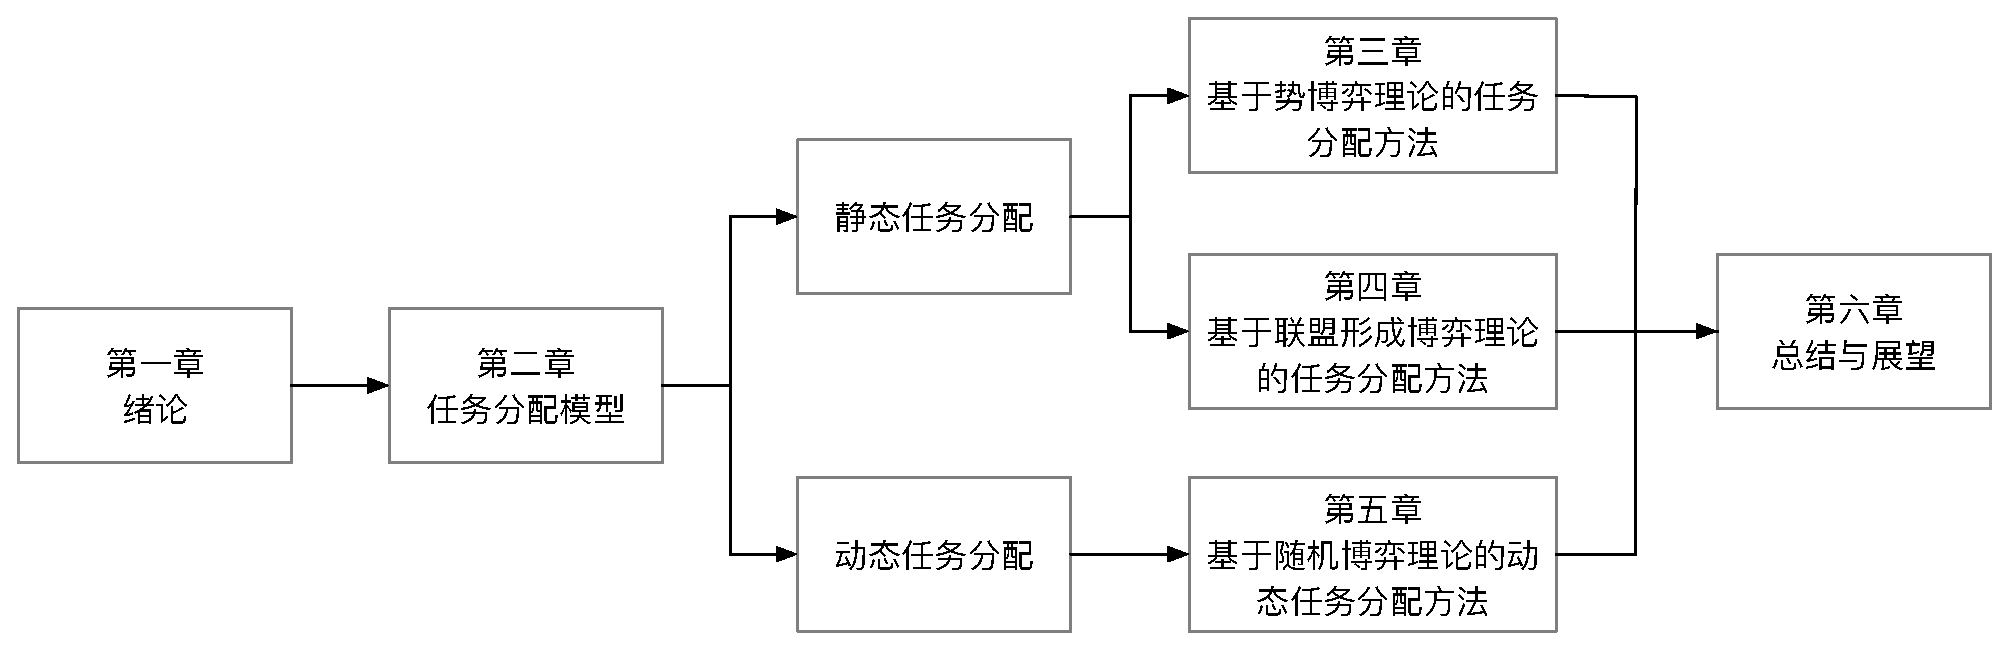
\includegraphics[height=4.5cm]{论文结构.eps} \\
  \bicaption[论文章节结构安排]
    {论文章节结构安排}
    {Structure arrangement of thesis chapters}
 \label{fig:structure}
\end{figure}

第\ref{chap:intro}章为绪论部分,首先介绍了选题背景等相关知识,简要阐述了集群空战背景下任务分配技术发展的必要性,对分布式任务分配技术的优缺点进行了归纳,并对基于博弈论思想的任务分配方法做了简要的梳理与分析,为后序博弈模型的建立和算法的设计做了铺垫。

第\ref{chap:model}章为空空导弹任务分配模型,建立了某一时间点的静态任务分配模型和一段时间的动态任务分配模型两种模型。针对静态任务分配模型,从空空导弹的特性出发,以最小化总攻击时间和最小化导弹机动量为目标,基于混合整数规划模型建立了多对多任务分配模型。针对动态任务分配模型,引入了导弹探测半径与通信半径的概念,建立了导弹对目标的探测模型以及导弹之间的通信模型,从而建立起动态场景下的任务分配模型。

第\ref{chap:pg}、\ref{chap:hedonic}章研究了针对某一时间点的分布式静态任务分配模型及其算法。

第\ref{chap:pg}章研究了基于势博弈理论的分布式任务分配方法,基于势博弈理论,基于Lagrange乘子法改进了WLU效用函数,建立了带约束条件的混合整数规划任务分配模型,通过数学推导证明了改进效用函数的有效性及性能下界。使用并比较了三种针对势博弈模型的分布式协商策略算法的有效性与性能,并改进了SAP算法,通过与集中式启发式算法的仿真对比实验,验证了设计模型与算法的有效性。

第\ref{chap:hedonic}章基于偏好联盟博弈理论,将任务分配问题看作联盟划分问题,设计了针对联盟划分问题的联盟效用函数,建立了带约束条件的偏好联盟博弈任务分配模型。从理论上推导出该模型的性能下界,得到了提高模型性能的方法。针对该模型设计了针对偏好联盟博弈模型的协商算法,改进了SAP使其适应于偏好模型,并使用DMEA算法求解。通过仿真实验验证了提出模型和算法的有效性。

第\ref{chap:stochastic}章研究了动态场景下的分布式任务分配模型及其算法。基于随机博弈理论,将导弹攻击过程划分为若干博弈子阶段,并在每个阶段建立\ref{chap:pg}、\ref{chap:hedonic}章建立的静态模型并求解。为了博弈子阶段之间的切换连贯,设计了子阶段分配前初始解的交叉生成机制和分配后新解的惰性机制。针对导弹通信网络非连通,以及目标数量发生变化两种场景进行分析并相应设计了重分配触发机制。最后通过场景仿真验证了所提出的动态分配框架的有效性,且对于动态环境有较好的应变能力。

第\ref{summary}章总结了全文的主要工作和主要贡献,并指出了本文的不足,对下一步工作也提出了展望。







